\section{Our Approach}

\subsection{Using FastText}

The methods described above are quite simple. We also compare the above method with FastText, which is a library for creating word embeddings developed by Facebook~\cite{BagOfTricks}. 

In the paper "Enriching Word Vectors with Subword Information" \cite{EnrichingWordVectors} the authors explain how FastText extracts feature vectors from raw text data. FastText makes word embedding using one of two model architectures: continuous bag of words (CBOW) or the continuous skip-gram model.

The skip-gram and CBOW models are first proposed in \cite{EfficientWordRepresentations} which is the paper introducing the word2vec model for word embeddings. FastText builds upon this work by proposing an extension to the skip-gram model which takes into account sub-word information.

Both models use a neural network to learn word embedding from using a context windows consisting of the words surrounding the current target word. The CBOW architecture predicts the current word based on the context, and the skip-gram predicts surrounding words given the current word.\cite{EfficientWordRepresentations}

\subsection{Using A Convolutional Neural Network}

While every layer in the MLP is densely connected such that each of the nodes in a layer is connected to all nodes in the next layer, in a convolution neural network we use one or more convolutional layers.

Convolutional Neural networks are very popular for image recognition but they can also be used for text classification \cite{textcnn_google}.

\begin{figure}[h!]
  \centering
  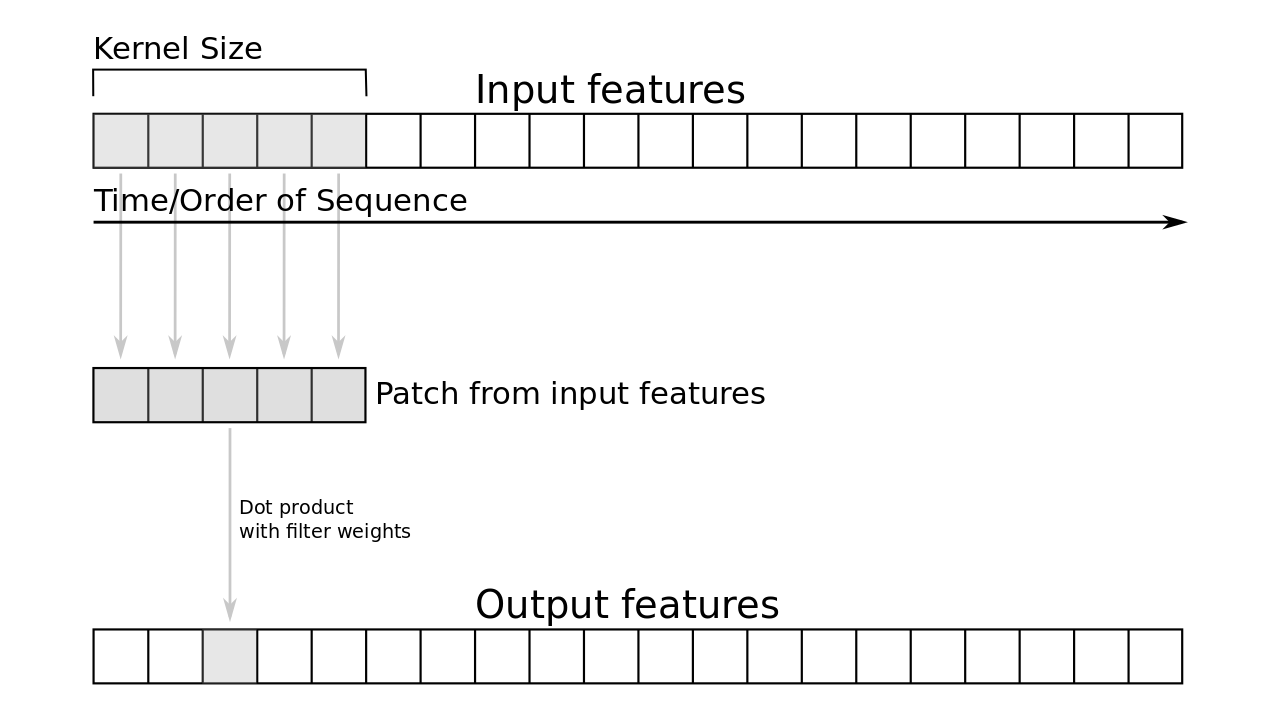
\includegraphics[width = 200pt]{figs/cnn_diagram}
  \caption{Diagram of Convolutional Neural network.}
  \label{cnn}
\end{figure}

The basic premise of a convolutional layer is illustrated in Figure~\ref{cnn}.\footnote{Source: \url{https://realpython.com/python-keras-text-classification/}} In a CNN you have a filter which slides over the input. The CNN then takes the dot product of the weights of the filter and the corresponding input features, before applying the activation function.
